\chapter{Empurrando Juntos} \label{cap:empurrandojuntos}

O uso da tecnologia tem auxiliado no aumento da participação dos 
cidadãos no âmbito político e social de diversas maneiras. Discussões em sites, principalmente redes sociais, têm sido
destaques como uma forma recorrente desta participação \cite{marques2008participaccao}.
Contudo, considerando as características das plataformas utilizadas e a existência de grupos dominantes, interessados
na área passaram a observar um viés nas mensagens trocadas \cite{empurrandojuntos, marques2008participaccao}. 

O ``Empurrando Juntos'' surge nesse contexto, como uma plataforma capaz de contornar a situação de polarização nas discussões.
A ideia apresentada pelo Instituto Cidade Democrática tem como objetivo dar voz para a minoria e 
melhorar a efetividade dos debates e conversas de acordo com o seu propósito, possibilitando ao usuário
identificar grupos de opinião e tendências em uma conversa. Além disso, como diferencial de outras aplicações
incluem ainda a gamificação a fim de promover a interação entre os membros agrupados em uma mesma classe 
\cite{empurrandojuntos}. 

\begin{figure}[h!]
\centering
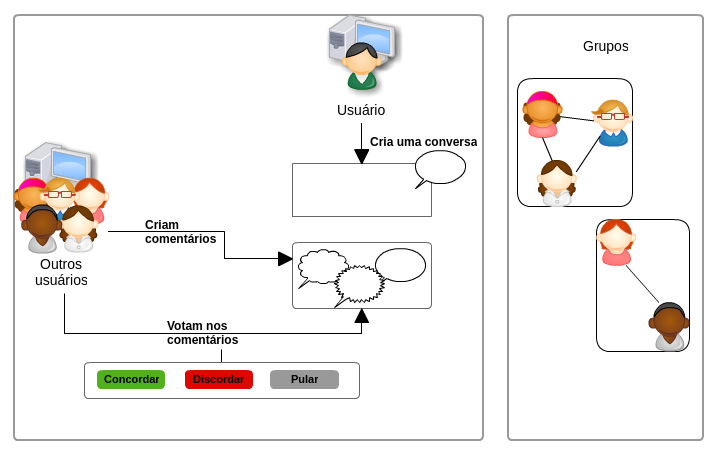
\includegraphics[scale=0.7]{figuras/resumo_ej.png}
\caption{Funcionamento do ``Empurrando Juntos''}
\label{fig:resumo_ej}
\end{figure}

A Figura \ref{fig:resumo_ej} ilustra o funcionamento completo do sistema. O usuário entra no sistema e pode criar conversas ou
comentar em conversas criadas por outros usuários. Para cada comentário realizado nessas conversas, é possível atribuir um 
``voto'' de concordância ou discordância do conteúdo exposto. Os votos são entendidos como a opinião dos usuários e são
utilizados para a formação dos grupos de opiniões. 

Em relação a gamificação proposta, \citeonline{empurrandojuntos} criaram o conceito de ``the Push'' que consiste
em prover notificações para determinados usuários e concedê-los o poder de enviar mensagens e criar eventos. Com 
o intuito de movimentar ainda mais as participações na aplicação e criar comunicação entre os usuários agrupados.

\citeonline{parra}, em um artigo para a página do Instituto Cidade Democrática apresenta os três perfis de usuário
que receberão essas notificações:

\begin{enumerate}
  \item \textbf{Ativista de minoria}: usuários com representação em um grupo de minoria, ou seja, que não concordam com a opinião 
    expressa em maior volume;
  \item \textbf{Pessoa ponte de diálogo}: usuários com opiniões ``contraditórias'', que normalmente concordam com a maioria, mas
    possuem alguns pensamentos diferentes demonstrando compatibilidade com outros grupos;
  \item \textbf{Criador da consulta}: usuários específicos representantes de consultas de governos para auxiliar na criação de projetos
  e políticas.
\end{enumerate}


Contudo, a ideia da utilização dessas notificações e perfis ainda necessita de validações e deverá ser bem
acompanhada para garantir a efetividade do seu propósito \cite{empurrandojuntos, parra}. 

Levando isto em consideração, o escopo inicial do sistema foi definido em um mapa mental, apresentado na Figura \ref{fig:mapa_mental_ej}. 
A princípio, a ferramenta deve fornecer o gerenciamento de usuários, com cadastro, atualização, exclusão e autenticação, 
incluindo contas provenientes do Facebook. Além disso, deve prover funcionalidades para o gerenciamento das conversas, comentários
e votos. Por fim, deve prover também a funcionalidade principal de agrupamento dos usuários de acordo com os votos obtidos.

\begin{figure}[h!]
\centering
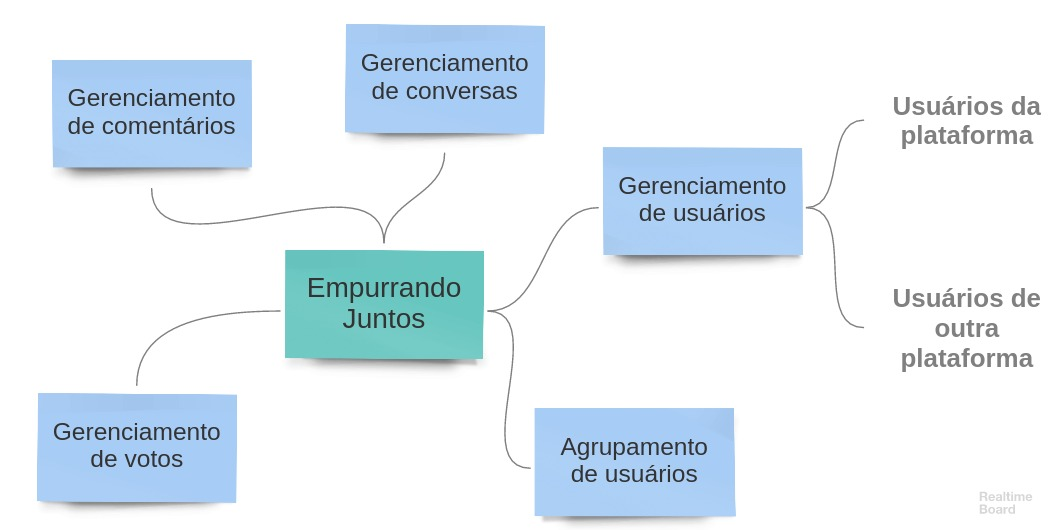
\includegraphics[scale=0.35]{figuras/mapa_mental_ej.jpg}
\caption{Escopo da plataforma}
\label{fig:mapa_mental_ej}
\end{figure}


Tal agrupamento pode ser implementado utilizando técnicas de classificação de dados.
De acordo com a proposta descrita por \citeonline{empurrandojuntos}, 
em um primeiro momento, essa classificação seria realizada utilizando algoritmos de clusterização. 

Em suma, o objetivo da plataforma é realizar o agrupamento de pessoas que responderam de maneira parecida, ou seja, 
concordaram e discordaram dos mesmos comentários. Com os grupos formados, a convergência e divergência 
de opiniões e uma visualização mais efetiva da opinião das pessoas são apresentadas aos usuários. 

Nesse sentido, este trabalho 
é uma contribuição para o ``Empurrando Juntos'' por meio da proposta e implementação de uma API para expor como serviços as funcionalidades
relacionadas ao escopo apresentado na Figura \ref{fig:mapa_mental_ej}  e permitir o uso de diferentes técnicas 
de classificação de dados.


